\section{Fazit}

In diesem Kapitel wird die von uns analysierte Hardware und Software noch
mal zusammengefasst, miteinander vergliechen und bewertet. Basierend
auf diesen Ergebnissen wird jeweils eine Empfehlung f"ur Hardware und
Software gegeben. Auf Basis dieser Empfehlungen soll es m"oglich sein,
ein WMN aufzubauen, das alle wichtigen Anforderungen aus Kapitel
\ref{sec:Aufgabenstellung} erf"ullt.

\subsection{"Ubersicht und Bewertung analysierter Hardware}

\begin{table}
\centering
\setlength{\extrarowheight}{4pt}
\capstart
\begin{tabular}{|p{4cm}|c|c|c|c|c|c|c|c|c|}
\hline
% HEAD BEGIN
 &
\rotatebox{90}{IEEE 802.11abgn} & \rotatebox{90}{Ad-Hoc Modus} &
\rotatebox{90}{Treiber (Linux/Windows)} & \rotatebox{90}{Open-Source Firmware} &
\rotatebox{90}{LAN-Anschluss} & \rotatebox{90}{Sicherheit} &
\rotatebox{90}{Installation} & \rotatebox{90}{Konfiguration} &
\rotatebox{90}{MiniPCI Slot}\\
% HEAD END
\hline
Linksys WMP55AG                  & ++  & + & ++ & -   & ++ & ++  & ++ & + & - \\
\hline
Netgear WAG311                   & ++  & + & ++ & -   & ++ & ++  & ++ & + & - \\
\hline
D-Link DWL-A520                  & +   & + & ++ & -   & ++ & +   & ++ & + & - \\
\hline
Gigabyte GN-WPEAG                & ++  & + & ++ & -   & ++ & +++ & ++ & + & - \\
\hline
Intel PRO/Wireless 5000          & +   & + & +  & -   & ++ & +   & ++ & + & - \\
\hline
D-Link DWL-AG530                 & ++  & + & ++ & -   & ++ & +++ & ++ & + & - \\
\hline
D-Link DWL-G550                  & ++  & + & ++ & -   & ++ & +++ & ++ & + & - \\
\hline
\hline
Wistron CM9 Atheros AR5213A      & ++  & + & ++ & -   & ++ & +++ & ++ & + & - \\
\hline
Intel PRO/Wireless 3945          & ++  & + & ++ & -   & ++ & +++ & +  & + & - \\
\hline
Intel PRO/Wireless 2915          & ++  & + & ++ & -   & ++ & +++ & +  & + & - \\
\hline
Intel Wireless WiFi Link 4965AGN & +++ & + & ++ & -   & ++ & +++ & +  & + & - \\
\hline
\hline
Linksys WRT54G v1.0              & ++  & + & -  & ++  & +  & +++ & -  & + & + \\
\hline
Linksys WRT55AG                  & ++  & + & -  & +   & +  & +   & -  & + & ++ \\
\hline
Asus WL500G/GP                   & ++  & + & -  & +++ & +  & +++ & -  & + & + \\
\hline
Netgear HR314                    & +   & - & -  & -   & +  & +   & -  & + & - \\
\hline
\end{tabular}
\caption{"Ubersicht und Bewertung analysierter Hardware}
\label{fig:"Ubersicht und Bewertung analysierter Hardware}
\end{table}

Auf Abbildung \ref{fig:"Ubersicht und Bewertung analysierter Hardware}
kann man von uns analysierte Hardware in tabellarischer Form noch mal
betrachten. Alle bei der Analyse wichtige Eigenschaften der Hardware
werden in der Tabelle zusammengefasst und bewertet.

Folgende Eigenschaften analysierter Hardware spielten bei der Bewertung
eine wichtige Rolle:

\begin{itemize}
\item Unterst"utzung f"ur IEEE 802.11a Standard
\item Unterst"utzung f"ur Ad-Hoc Modus im 5 GHz Frequenzbereich
\item Vorhandensein von Treibern sowohl f"ur Linux als auch Windows
\item Vorhandensein von Open-Source Firmware f"ur SoHO-Router
\item Vorhandensein der LAN-Schnittstelle
\item Unterst"utzung f"ur Verschl"usselung
\item Schwierigkeitsgrad der Installation
\item Schwierigkeitsgrad der Konfiguration
\item Vorhandensein von MiniPCI-Slots bei SoHO-Routern
\end{itemize}

Die analysierte Hardware wurde in 2 Kategorien aufgeteilt. Die Hardware
aus der ersten Kategorie kann in PCs eingesetzt werden, ohne PCs ist diese
Hardware als Mesh-Router nicht verwendbar. Die Hardware aus der zweiten
Kategorie sind WLAN SoHO-Router, diese Hardware muss auch angepasst werden,
denn die meisten SoHO-Router den Standard IEEE 802.11a und Ad-Hoc Modus
im 5 GHz Frequenzband nicht unterst"utzen. In Tabelle
\ref{fig:"Ubersicht und Bewertung analysierter Hardware} wurde die analysierte
Hardware aber in 3 Gruppen aufgeteilt: PCI WLAN-Karten, MiniPCI(e) WLAN-Karten
und SoHO WLAN-Router. Die MiniPCI WLAN-Karten k"onnen in Mesh-Routern auf
PC-Basis eingesetzt werden, m"ussen aber nicht. Manche SoHO WLAN-Router
brauchen aber mindestens eine MiniPCI WLAN-Karte, die Ad-Hoc Modus
im 5 GHz Frequenzband unterst"utzt, denn die meisten von uns analysierten
SoHO WLAN-Router k"onnen nur im 2.4 GHz Frequenzband funktionieren.
Deswegen muss ihre alte MiniPCI WLAN-Karte gegen eine ersetzt werden,
die auch im 5 GHz Frequenzband funktionieren kann.


\subsection{"Ubersicht und Bewertung analysierter Routing-Software}

\begin{table}
\centering
\setlength{\extrarowheight}{4pt}
\capstart
\begin{tabular}{|l|c|c|c|c|c|}
\hline
% HEAD BEGIN
 &
\rotatebox{90}{Betriebssysteme} & \rotatebox{90}{Installation} &
\rotatebox{90}{Konfiguration} & \rotatebox{90}{Visualisierung} &
\rotatebox{90}{Open-Source}\\
% HEAD END
\hline
OLSRD        & +++ & + & + & ++ & +\\
\hline
B.A.T.M.A.N. & +   & + & + & -  & +\\
\hline
Meshcom      & +   & + & - & +  & -\\
\hline
\end{tabular}
\caption{"Ubersicht und Bewertung analysierter Routing-Software}
\label{fig:"Ubersicht und Bewertung analysierter Routing-Software}
\end{table}

Auf Abbildung \ref{fig:"Ubersicht und Bewertung analysierter Routing-Software}
kann man von uns analysierte Routing-Software in tabellarischer Form noch mal
betrachten. Alle bei der Analyse wichtige Eigenschaften der Routing-Software
werden in der Tabelle zusammengefasst und bewertet.

Folgende Eigenschaften analysierter Routing-Software spielten bei der Bewertung
eine wichtige Rolle:

\begin{itemize}
\item Unterst"utzung sowohl f"ur Linux als auch f"ur Windows
\item Schwierigkeitsgrad der Installation
\item Schwierigkeitsgrad der Konfiguration
\item Unterst"utzung f"ur Visualisierung von Topologie
\item Frei verf"ugbarer Quellcode
\end{itemize}

\subsection{Empfehlung f"ur Hardware und Software}

In diesem Abschnitt wird eine Empfehlung sowohl f"ur Hardware als auch
f"ur Routing-Software gegeben. Diese Empfehlungen basieren auf unserer
Analyse und Bewertung im vorherigen Abschnitt. Ausserdem werden genaue Gr"unde
f"ur unsere Empfehlungen genannt.

\subsubsection{Empfehlung f"ur Hardware f"ur Mesh-Router}

In diesem Abschnitt geben wir unsere Empfehlung f"ur Hardware zum Einsatz in
Mesh-Routern eines WMNs.

Als Hardwareplattform f"ur Mesh-Router empfehlen wir den Einsatz von PCs mit
mehreren PCI bzw. MiniPCI WLAN-Karten mit Atheros Chipsatz und einer
LAN-Schnittstelle. Welche PCI oder MiniPCI WLAN-Karten dabei eingesetzt
werden sollen, haben wir nicht entschieden, denn sie haben alle fast
"ahnliche Eigenschaften und alle analysierten WLAN-Karten mit Atheros
Chipsatz werden herrvorragend von MadWifi-Treiber unterst"utzt.
Jede von uns analysierte PCI oder MiniPCI WLAN-Karte mit Atheros
Chipsatz ist f"ur den Einsatz in Mesh-Routern gut geeignet, wir empfehlen
aber den Einsatz von Wistron CM9 Atheros AR5213A WLAN-Karte
(siehe \ref{Wistron CM9 Atheros AR5213A}), weil sie von uns pers"ohnlich
im Labor erfolgreich mit MadWifi-Treibern getestet wurden.
Ausserdem ist Wistron CM9 Atheros AR5213A MiniPCI WLAN-Karte auch
in SoHO WLAN-Routern einsetzbar.

Als Betriebsystem f"ur Mesh-Router empfehlen wir nat"urlich Linux.
F"ur Linux existieren sehr viele Programme zur Analyse und Evaluierung
von drahtlosen Netzwerken. Ausserdem bietet Linux einen sehr m"achtigen
Packet Filter iptables. Zus"atzlich existieren daf"ur sehr viele Open-Source
Programme wie HTTP-, SSH- und DHCP-Server, die man beim Aufbau eines WMN sehr
gut gebrauchen kann, was wir auch bei unseren Tests gemacht haben.
Wir haben z.B. Apache HTTP-Server f"ur die Visualisierung der Topologie
unseres kleinen WMN verwendet. F"ur Linux existiert eine Menge von
Skript-Sprachen wie z.B. Perl, Python, die viele Verwaltungsaufgaben
in einem WMN erleichtern k"onnen. Und schliesslich existiert f"ur Linux
sehr gute Dokumentation im Internet.

Aus folgenden Gr"unden haben wir uns f"ur den Einsatz von PCs mit
WLAN-Karten und nicht f"ur den Einsatz von SoHO-Routern entschieden:

\begin{itemize}
\item PCs sind nicht sehr teuer, daf"ur aber sehr flexibel.
\item PCs sind sehr flexibel, sie haben viel mehr Speicher als SoHO-Router
und sind leicht erweiterbar. Man kann theoretisch unbegrenzt viele Software-Tools
zur Verwaltung und zur Evaluierung von WMNs installieren.
\item SoHO-Router m"ussen erstmal umgebaut werden, denn keiner von uns
analysierten SoHO-Routern unterst"utzt Ad-Hoc Modus im 5 GHz Frequenzband.
\item Auf SoHO-Routern muss eine Open-Source Firmware installiert werden.
\item SoHO-Router haben sehr wenig Speicher zur Verf"ugung und machen
den Einsatz mancher Software-Tools unm"oglich.
\item PCs sind nicht nur als Mesh-Router einsetzbar.
\item Beliebige Linux-Distributionen k"onnen installiert werden.
\end{itemize}

\subsubsection{Empfehlung f"ur Routing-Software}

In diesem Abschnitt geben wir unsere Empfehlung f"ur Routing-Software
zum Einsatz in Mesh-Routern eines WMNs.

Als Routing-Software, die in den Mesh-Routern eines WMNs zum Einsatz kommt,
empfehlen wir den Einsatz von Routing-Daemon von olsr.org. Beim OLSR
Routing-Daemon von olsr.org sollten keine Skalierbarkeitsprobleme auftreten,
da abgesch"atzte Anzahl von Mesh-Routern im WMN niedrig ist. Ausserdem
unterst"utzt der Routing-Daemon von olsr.org Visualisierung von Topologie.
Er unterst"utzt sowohl Linux als auch Windows und ist in beiden
Betriebssystemen sehr leicht zu installieren und zu konfigurieren.

Vom Einsatz von B.A.T.M.A.N. raten wir ab, der Routing-Daemon von
B.A.T.M.A.N. unterst"utzt noch keine Visualisierung von Topologie
und das Routing-Protokoll B.A.T.M.A.N.  befindet sich zur Zeit immer
noch in Entwicklung.  Ausserdem unterst"utzt der Routing-Daemon von
B.A.T.M.A.N. das Betriebssystem Windows nicht.

Den Einsatz von Meshcom empfehlen wir auch nicht, denn sowohl das
Protokoll als auch der Routing-Daemon sind nicht frei verf"ugbar.
Der Routing-Daemon von Meshcom ist nicht kostenlos. Wir haben nur mit
einem Demo-Programm getestet.

\subsubsection{Aufbau von WMN}
\label{sec:Aufbau}

\begin{figure}[H]
\centering
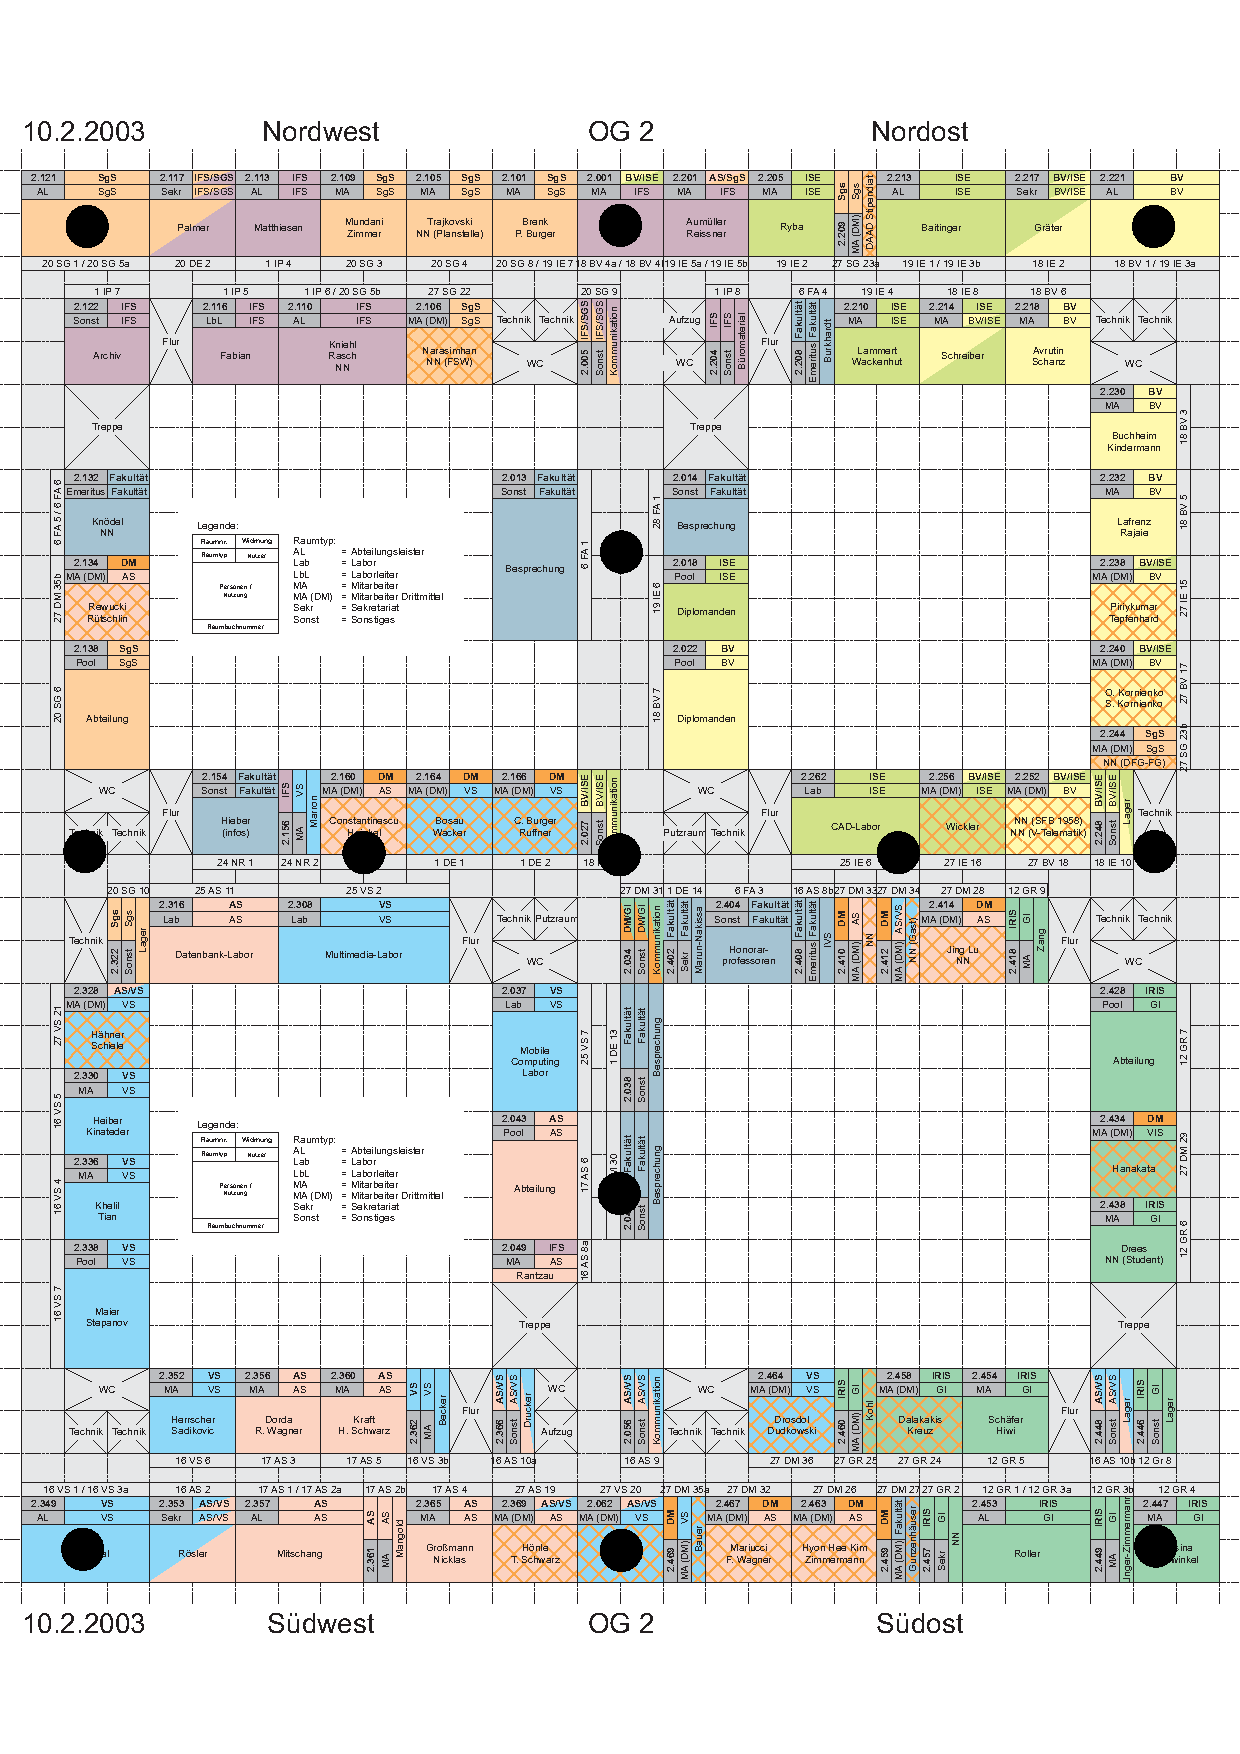
\includegraphics[width=0.8\textwidth]{images/plan.pdf}
\caption{M"ogliche Plazierung von Mesh-Routern im Informatik Geb"aude}
\label{fig:plan}
\end{figure}
	
Um das ganze Informatikgeb"aude abzudecken, w"urden ca. 27-39 PCs reichen.
Das heisst ca. 9-13 PCs pro Stock.  Auf Abbildung \ref{fig:plan} ist
eine m"ogliche Plazierung von Mesh-Routern zu sehen.  Kosten f"ur die
notwendige Hardware liegen damit unter der Budget-Grenze.
